\documentclass[a4paper]{jpconf}
\usepackage{graphicx}
\usepackage{url}
\usepackage{hepparticles}
\usepackage[nomargin,inline,marginclue,draft]{fixme}

\begin{document}
\title{A novel method for event reconstruction in Liquid Argon Time Projection Chamber}

\author{M Diwan, M Potekhin, B Viren, X Qian and C Zhang}

\address{Brookhaven National Laboratory, Upton, NY11973, USA}

\ead{xqian@bnl.gov}

%The Liquid Argon Time Projection Chamber (LArTPC) has the potential to provide exceptional level of detail
%in studies on neutrino interactions - a high prioritory field of Intensity Frontier research. Liquid Argon serves as both
%the target for neutrino interactions and the sensitive medium of the detector, which measures ionization produced by
%the reaction products. The LArTPC has characteristics suitable for precise reconstruction of infividual tracks as well
%as for calorimetric measurements. In order to gain sensitivity to reactions with very small cross-sections, modern
%LArTPC devices are built at a considerable scale, currently in hundreds of tons of instrumented volume of Liquid Argon.
\begin{abstract}
Future experiments such as the Deep Underground Neurtino Experiment (DUNE) will use very large Liquid Argon Projection Chambers
(LArTPC) containing tens of kilotons of cryogenic medium. To be able to utilize sensitive volume  of that size,
%that large while staying within practical limits of power consumption and cost of the front-end electronics,
current design employs arrays of wire electrodes
grouped in readout planes, arranged with a stereo angle. This presents certain challenges for object reconstruction
due to ambiguities inherent in such scheme. We present a novel reconstruction method (named ``Wirecell') inspired by principles
used in tomography, which brings the LArTPC technology closer to its full potential.

\end{abstract}


\section{Introduction}

The new method of event reconstruction in Liquid Argon Time Projection Chamber (LArTPC) presented here
is motivated by the stringent requirements of the DUNE experiment~\cite{cdrVol1}. The DUNE primary science
program~\cite{cdrVol2} includes
\begin{itemize}
\item precision measurements of the parameters that govern \HepParticle{\nu}{\mu}{} $\rightarrow$ \HepParticle{\nu}{e}{} and
 \HepAntiParticle{\nu}{\mu}{} $\rightarrow$ \HepAntiParticle{\nu}{e}{} oscillations
\item search for proton decay in several important decay modes, for example \HepParticle{p}{}{} $\rightarrow$ \HepParticle{K}{}{+}\HepAntiParticle{\nu}{}{}
\item detection and measurement of the \HepParticle{\nu}{e}{} flux from a core-collapse supernova in our galaxy, should any occur during the lifetime
of the DUNE experiment
\end{itemize}
\noindent
DUNE has been conceived around three central components: an intense wide-band neutrino beam originating at FNAL; a fine-grained Near Neutrino Detector
just downstream of the neutrino source; and a a massive Far Detector (40kt fiducial volume) based on Liquid Argon Time Projection Chamber located deep
underground at a distance of 1,300\,km from the neutrino source~\cite{cdrVol4}.

The  Liquid Argon Time Projection Chamber (LArTPC)  has the potential to reconstruct tracks and showers with high high level of detail and high efficiency,
as well as to provide a precise measurement of ionization charge necessary for good particle identification based on ionization energy loss ($dE/dx$).
The single-phase LArTPC design which is our focus here is essentially an ionization chamber with multi-wire readout and no amplification in the medium,
which is cryogenic liquid Argon. There are a number of differences between Time Projection Chambers used in collider and other experiments, and current generation
of large LArTPCs developed for Intensity Frontier. In LArTPC:

\begin{itemize}
\item liquid argon serves as both the target and the sensitive medium

\item there are no axiliary detectors e.g. ``inner tracker'' and/or dedicated calorimeters

\item the event vertex is  located inside the LArTPC itself
%and its position is not constrained
%since the interaction can happen anywhere in the sensitive volume; this is not the case with TPCs in collider experiments

\item there is no magnetic field, so it can't be used to estimate the particle momentum

\item for a very large detector like DUNE using pads for readout is not practical, and the liquid argon volume is instrimented with planar arrays of wire
electrodes

\end{itemize}
%\noindent
%The latter point is important because it leads to the design choice where  This impacts approaches that can be utilized in event reconstruction, as will be explained in
%the following sections.

%%%%%%%%%%%%%%%%%%%%%%%%%% principles %%%%%%%%%%%%%%%%%%%%%%%%%%
\section{Operation of the LArTPC with wire readout}
\subsection{Wire Planes}
The LArTPC volume is instrumented with sensor wires which in case of DUNE are spaced at a $\sim$4.5\,mm pitch, and configured 
asl planar arrays forming induction and collection planes. The planes are aggregated into structural units called ``Anode Plane Assemblies'',
or APAs. Each side of the APA contains two induction planes and one collection plane, in a stereo angle configuration. This is illustrated in
Fig.\ref{fig:wireplanes1} which is a schematic view of the APA along the drift direction (i.e. line of sight is perpendicular to the APA).
\begin{figure}[h!]
	\centering
	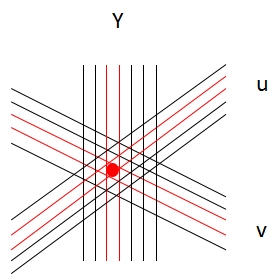
\includegraphics[width=0.5\textwidth]{wireplanes1.png}
	\caption{Collection and Induction Wire Planes as viewed along the drift direction}
	\label{fig:wireplanes1}
\end{figure}

\noindent
In this diagram, arrays of wires labeled ``u'' and ``v'' represent the two induction planes, while ``Y'' wires constitute the
collection plane, i.e. the electrodes where ionization electrons are collected after completing their drift in the liquid argon medium.
Every induction and collection wire is read out as an individual channel, with waveforms recorded at $\sim$2\,MHz digitization frequency.
There are also planar ``Cathode Plane Assemblies'' which are necessary to create a proper near-uniform electrostatic field in
the chamber, however they are not instrimented.
\subsection{General Principle of Operation}
The LArTPC principle of operation of  is schematically illustrated in Fig.\ref{fig:lartpc-principle}.
In this diagram, ionization electrons are
produced in the medium by a few tracks associated with an event. They start drifting to the right, while
positive ions travel towards the cathode on the left hand side. Drifting electrons come produce signals on the induction wires (in planes ``U''
and ``V''). Signals will also be created on the collection wire plane ``Y'' once the electrons are in its vicinity. The ionization pattern can then be recontructed
 in the plane perpendicular to the drift direction by analyzing signals on ``U'' and ``V''. 
\begin{figure}[h!]
	\centering
	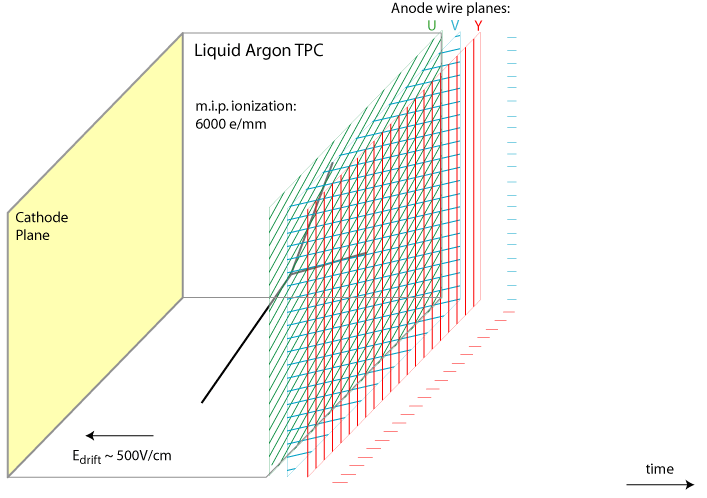
\includegraphics[width=0.8\textwidth]{signal-0.png}
	\caption{The LArTPC Principle of Operation}
	\label{fig:lartpc-principle}
\end{figure}
Reconstroction along the axis of the drift direction
can be done using the information contained in the time evolution of the signals on UVY wire planes, since each time bin corresponding to the
ADC digitization cycle can be mapped to the coordinate in that direction, through the known (calibrated) value of drift velocity.

In general, signals on individual wires produce complex waveforms, and are subject to electronics noise, shaping parameters in the
amplifier chain and other factors. Evaluating the charge in a particular time bin involves complex signal processing, and
is beyond the scope of this paper.

\subsection{The Challenge}
\label{ambiguity}
It is not difficult to see that the while the wire readout design makes construction of large LArTPCs practical by keeping the channel count
in check, it does so at the cost of certain information loss, since now instead of pads or pixels one has to reconstruct the position of the
particle ``hits'' in 2D using just three projections. The situation is somewhat similar to the well-known phenomenon of ``ghost hits'' which
previously existed in certain detector systems in HEP, with multiwire and/or strip-based readout. If the number of sensor wires that
registered a signal is $\sim$N, the number of potential hit locations scales as $\sim$N$^2$, which naturally leads to ambiguities.



\section{The ``Wirecell'' method}
\subsection{Reconstruction in LArTPC}
Event reconstruction in LArTPCs with wire readout is not straightforward.
Reconstruction methods which existed prior to introduction of the method described in this paper were inspired by tracking
algorithms utilized in High Energy Physics (and collider experiments in particular), and indeed reused existing software libraries
in some cases. A typical approach would start with identifying track candidates in each of the three projections which were described
above. This is done by identifying groups of wires in each projection which had ``hits'' is adjacent time bins, effectively relying
on the continuity of the object being reconstructed at this stage in the reconstruction process. Hypotheses are applied regarding
whether the object coresponds to a track or to a shower. Then, an attempt is made to match individual 2D (time-coordinate)
projections in 3D. As mentioned in \ref{ambiguity}, there are inherent ambiguities in this process, which ultimately manifest themselves as
reconstruction artifacts such as ghost tracks etc. Detailed analysis of this problem area is beyond the scope of this paper.


\subsection{Parallels to Tomography}
The very method of collecting signals from LArTPC has deep parallels with Computerized Axial Tomography
(CAT) applications. Namely, each time slice in LArTPC is
digitized separately and effectively represents a separate unit of data. This can be compared to one of the original (and simplest) methods of CAT
called Multiplanar Reconstruction -- MPR -- in which the volume under study is treated as a stack of 2D slices. Further, revisiting
Fig.\ref{fig:wireplanes1} one can see that the same charge pattern in an individual 2D slice is sampled in three different projections.
Each wire is effectively measuring a line integral of the ionization charge located in its vicinity. This has significant similarity
to absorption tomography where attenutation of radiation intensity also effectively corresponds to a line integral along
the direction of the beam. Clearly, the number of projections is extremely limited (to three) which makes application of ``mainstream''
CAT reconstruction techniques such as Radon transform ~\cite{radon1}
not practical. It must be noted however that ``sparse'' and ``limited-angle'' tomography
does have its applications and domain-specific mathematical methods have been developed to deal with such extremely ill-posed problems.

CAT applications typically feature voxelization of the object under study due to natural granularity of the apparatus and also to make numerical
calculations feasible. In multiplane reconstruction, this effectively leads to treating each individual 2D slice as a set of pixels, defined according
to the type of measurement. Application to this technique (introduction of ``cells'') is the foundation of the ``Wirecell'' method described here
\cite{wirecell} which is reflected in the method's name.

\subsection{The ``Wirecell'' algorithm}
In Wirecell, a tesselation algorithm is used to describe each 2D slices (defined by a particular time bin of the ADCs digitizing signals
collected from the LArTPC) as a set of polygons, effectively pixels. Each wire is associated with a particular subset of pixels which overlap
with the wire. Wirecell includes two essential steps:
\begin{itemize}
\item Solving the inverse problem in each 2D slice, i.e. performing 2D imaging (reconstructing pixel values) using the three projections of the
charge ``image'' available in the measurement
\item Combining the 2D slices to obtain a 3D model of the ionization pattern in the Liquid Argon Volume, which can them be used to extract
physics information about the event being studied
\end{itemize}

\noindent
The inverse problem of determining pixel values based on limited number of projections (three sets of wires) is an ill-posed one.
The following algorithm is applied: groups of adjacent candidate cells with signal above a certain
threshold are identified. They are grouped into ``merged cells'' (i.e. the charge values are combined to effectively form a larger pixel).
Note that many of these cells will be effectively ``ghosts'' due ambiguities as described above  (see~\ref{ambiguity}).
Wires mapped to these merged cells are also ``merged''. This results in reduction of the number of degrees of freedom. Signals on ``merged wires''
are what is observed experimentally, while the values of charge in merged cells are not due to ambiguities. The relationship
between the two can be represented as $W_m=G$\,$C_m$, where $W_m$ is the vector of values attributed to charges on merged wires, $G$ is
the geometry matrix mapping wires to cells, and the $C_m$ is the vector of values for merged cells, for which a solution must be found. In vast majority
of cases this cannot be solved by matrix inversion. Instead, the Wirecell method employes the Markov Chain Monte Carlo (MCMC) approach, which aims
to minimize the following value:
$$\chi^2=(W_m-GC_m)^TV^{-1}(W_m-GC_m)$$
Each step in the MCMC process involves removing a random cell and recalculating $G$ to evaluate the metric as described above. If the $\chi^2$ value
improves, such cell is permanently eliminated under the hypothesis that it was a ``ghost cell''. Once a sufficuent number of cells have been eliminated,
matrix inversion may become possible which completes the solution. A recontructed 2D image is formed, and a stack of these images forms the 3D
picture of the physics event in LArTPC.

Optimization technique as described above can be modified to take advantage of apriori information about the object, which is another common
approach in the field of tomography. For example the hypothesis of object continuity in 3D can be included in the solution by adding a penalty
value to $\chi^2$ in cases there there are no cells in neighboring 2D slices, adjacent to the one being considered for elimination during the MCMC step.

The Wirecell algorithm contains a number of elements which are computationally intensive, e.g. each step in the Markov Chain involves recalculating
matrices and other operations. For that reason, work is currently under way to adapt Wirecell for use on modern parallel computing platforms,
including GPUs.

\subsection{Status and future directions}
The Wirecell method has been applied for reconstruction of a variety event classes using Monte Carlo data. In first round of analysis, efficiency of track reconstruction
in this method is at or above the levels stupulated by the requirements of the DUNE experiment.
It is currently being adapted for
event reconstruction in the $\mu$BooNE experiment~cite{uboone}, and results are expected to become available soon.

\section{Summary}
A novel reconstruction method has been developed which applies tomography principles to the domain of Liquid Argon Projection Chambers with
wire readout. Markov Chain Monte Carlo technique is used for the inverse problem solution in 2D, with a full 3D image formed as a stack of 2D slices.
First results are promising and the methods can bring the LArTPC technology closer to its full potential for physics research.


\section*{References}
\begin{thebibliography}{9}
\bibitem{cdrVol1} DUNE CDR Vol 1 -- The LBNF and DUNE Projects: \url{http://arxiv.org/abs/1601.05471}
\bibitem{cdrVol2} DUNE CDR Vol 2 -- The Physics Program for DUNE at LBNF: \url{http://arxiv.org/abs/1512.06148}
\bibitem{cdrVol4}  DUNE CDR Vol 4 -- The DUNE Detectors at LBN:F \url{http://arxiv.org/abs/1601.02984}
\bibitem{radon1}  William H. Press, `` Discrete Radon transform has an exact, fast inverse and generalizes to operations other than sums along lines'', Proceedings of the National Academy of Sciences of the United States of America, 19249–19254, doi: 10.1073/pnas.0609228103
\bibitem{wirecell} Wirecell: \url{http://www.phy.bnl.gov/wire-cell/}
\bibitem{uboone} $\mu$BooNE experiment: \url{http://www-microboone.fnal.gov}

\end{thebibliography}

\end{document}


